\documentclass[10pt,letterpaper]{article}
\usepackage[hmargin=0.6in,top=0.5in,bottom=0.65in,footskip=18pt]{geometry}
\usepackage[T1]{fontenc}
\usepackage{amsmath,amssymb}
\usepackage{newpxtext}
\usepackage[slantedGreek]{newpxmath}
\linespread{1.0}
\usepackage{xcolor,booktabs,array,enumitem,microtype,multicol}
\usepackage[most]{tcolorbox}
\usepackage[hidelinks]{hyperref}
\makeatletter
\renewcommand\section{\@startsection{section}{1}{\z@}{-9pt plus -2pt}{4pt}{\normalfont\large\bfseries\color{teal}}}
\makeatother
\definecolor{ink}{HTML}{25343D}
\definecolor{teal}{HTML}{176F78}
\definecolor{gold}{HTML}{A16623}
\definecolor{muted}{HTML}{65767D}
\definecolor{plum}{HTML}{7A3E6B}
\definecolor{sky}{HTML}{2F6690}
\setlength{\parindent}{0pt}\setlength{\parskip}{2.5pt}
\setlist[itemize]{leftmargin=15pt,itemsep=2pt,topsep=3pt}
\setlist[enumerate]{leftmargin=18pt,itemsep=2pt,topsep=3pt}
\hypersetup{pdftitle={The Lowest Note: a geometric theory of the Yang-Mills mass gap},pdfauthor={Bee Rosa Davis}}

% ---------------------------------------------------------------- status boxes
% \begin{claim}{STATUS}{Title} ... \end{claim}
% STATUS is one of: PROVED, PROVED (CITED), COMPUTED, CONDITIONAL, CONJECTURE, OPEN
\newcommand{\statuscolor}[1]{%
  \ifnum\pdfstrcmp{#1}{PROVED}=0 teal\else
  \ifnum\pdfstrcmp{#1}{PROVED (CITED)}=0 teal\else
  \ifnum\pdfstrcmp{#1}{COMPUTED}=0 sky\else
  \ifnum\pdfstrcmp{#1}{CONDITIONAL}=0 gold\else
  \ifnum\pdfstrcmp{#1}{CONJECTURE}=0 plum\else muted\fi\fi\fi\fi\fi}
\newcounter{claimno}
\newtcolorbox{claimbox}[2]{enhanced,breakable,colback=\statuscolor{#1}!4!white,colframe=\statuscolor{#1},
  boxrule=0pt,leftrule=2.2pt,arc=0pt,outer arc=0pt,left=5pt,right=4pt,top=2pt,bottom=2pt,
  before skip=3pt,after skip=3pt,fontupper=\small,
  before upper={{\sffamily\small\bfseries\color{\statuscolor{#1}}\theclaimno.\ #2\ \
    {\fboxsep=1pt\colorbox{\statuscolor{#1}}{\color{white}\scriptsize #1}}}\ }}
% \refstepcounter outside the box so that \label inside the box body gives the box number
\newenvironment{claim}[2]{\refstepcounter{claimno}\begin{claimbox}{#1}{#2}}{\end{claimbox}}
% marks where a section carries one of the five points of the theory
\newcommand{\spine}[1]{{\sffamily\small\bfseries\color{plum}Point #1 of the theory.}\ }
\newcommand{\evidence}[1]{\par\vspace{1pt}{\footnotesize\color{muted}\textbf{Evidence.} #1}}
\newcommand{\lines}[1]{{\sffamily\scriptsize\color{muted}[lines #1]}}

\begin{document}
\color{ink}
{\sffamily\small\color{teal} A NARRATIVE THEORY, NOT A PROOF \hfill 27 NOVEMBER 2026}\par\vspace{4pt}
{\fontsize{24}{28}\selectfont The Lowest Note\par}
\vspace{1pt}{\large A geometric theory of the Yang--Mills mass gap\hfill\normalsize Bee Rosa Davis\par}
\vspace{2pt}{\small\color{muted}\emph{This document supersedes my earlier Zenodo posting, which claimed a proof of the Yang--Mills mass gap. That claim is withdrawn. What follows is a theory, not a proof: my complete account, as of today, of what I believe the mass gap is.}\par}
\vspace{2pt}

% s0: the theory in one sentence and five points, and how to read the boxes. ASCII only.
\begin{quote}\small
\textbf{The theory.} The mass gap of Yang--Mills theory is the energy cost of the cheapest way for the field to lean
toward changing its topology. It is carried by an identified shape at every scale, protected from the fine grain by
asymptotic freedom, and inherited all the way out to infinite space. If the theory is true, it says five things.
\textbf{(1)~The gap has a name:} in a small room it is carried by Helike, a twisting shape of charge~2 under the room's rotation symmetry, or by
her competitor, a breathing shape of charge~0, and as the room grows the carrier changes only at exact, countable
switches (\S4--5). \textbf{(2)~Topology decides who is lightest:} the energy landscape of the room is the squared slope
of the Chern--Simons function, and the competitor is exactly the direction that points toward the other winding vacuum,
which would explain why the scalar glueball is lightest (\S5; proved in the reduced model, while the full theory waits on one uncomputed term). \textbf{(3)~Tensor and scalar trade places at a
calculable point,} $s_0^*(t)=(t+2)(\sqrt{t+8}-\sqrt t)/(4\sqrt t)$, which is $1.1436$ at $t=3$ at harmonic order; the switches registered at stronger coupling rise from it (\S5). \textbf{(4)~The
fine grain cannot erase the note:} the infinitely many fast modes, at leading order, only rename the coupling, which is
asymptotic freedom ($b_0=22/3$ matched to $10^{-4}$) (\S6). \textbf{(5)~The infinite world is the last room:} infinite
space is the end of a family of spheres, and the gap is a section over that family that never touches zero (\S7--8).
Simulations and perturbation theory already show that the gap exists, that the scalar glueball is lightest and that
asymptotic freedom holds. What would be new is the reason behind all three, and that they are one fact seen from three
sides.
\end{quote}

\textbf{How to read this.} This is a narrative theory, not a proof, told as one story from the problem (\S1)
to what the gap is (\S10). Every important statement, proved or not, sits in a numbered box whose label gives its
standing: \textcolor{teal}{\textbf{PROVED}} (by me) and \textcolor{teal}{\textbf{PROVED (CITED)}} (by others),
\textcolor{sky}{\textbf{COMPUTED}} (numerically, not proved), \textcolor{gold}{\textbf{CONDITIONAL}} (proved from a
named hypothesis), \textcolor{plum}{\textbf{CONJECTURE}}, and \textcolor{muted}{\textbf{OPEN}}. Each box names the lines
of my register of statements~\cite{ClosedSet} it covers, and no box is stronger than its line. All 29 lines (29 is
merged into 23) appear below; \S10 tabulates where. The finer evidence, mine and
others', is in the companion blog post and the repository~\cite{HelikeReport}.

% s1: the problem, as it is posed. ASCII only.
\section{Introduction: the problem and the proposal}

\subsection*{What I mean by Helike}

Before I follow Helike through this theory, I want to say what she is. Helike is the name I give to an explicitly
identified family of deformation modes of a Yang--Mills field on a Berger sphere: a three-sphere stretched along a
preferred family of circles. A mode tells me how the field changes, point by point. It is a pattern of field
variation, not a new particle placed inside the theory.

The Yang--Mills Hessian measures the quadratic energy variation about a background field. Its eigenvalue gives
a number; its eigenvector gives the pattern that number belongs to. My starting point is to follow that pattern,
not only its number. My earlier work identifies Helike exactly and establishes the domain in which she occupies
the bottom of that Hessian spectrum~\cite{ByEnough,Floor}. Here I ask what quantum dynamics makes of this geometric
mode: how it contributes to an excitation, competes with another shape, and responds to the finer modes and the
size of the space. A Hessian mode and a full quantum state are different objects; following the connection is part
of this theory.

In her simplest homogeneous form, Helike is a \emph{doublet}: two real patterns spanning one two-dimensional mode
space (Figure~\ref{fig:helike-doublet}). Their coefficients are constant in the moving frame; the frame itself varies
over the sphere. At a circle-symmetric background the two partners have the same Hessian eigenvalue.

\par\Needspace{7\baselineskip}
\emph{Charge 2} describes their rotation law, not electric charge. Rotate the spatial frame and the compensating
colour frame together through an angle $\theta$: the pair of coefficients turns through $2\theta$. A $45^\circ$
rotation takes the first pattern to the second; a $90^\circ$ rotation gives the negative of the first, not the same
pattern. A $180^\circ$ rotation returns it. This is the precise sense of the turn shown here, not a drawing of a
material ribbon or a trajectory through space.

\begin{figure}[!htbp]
\centering
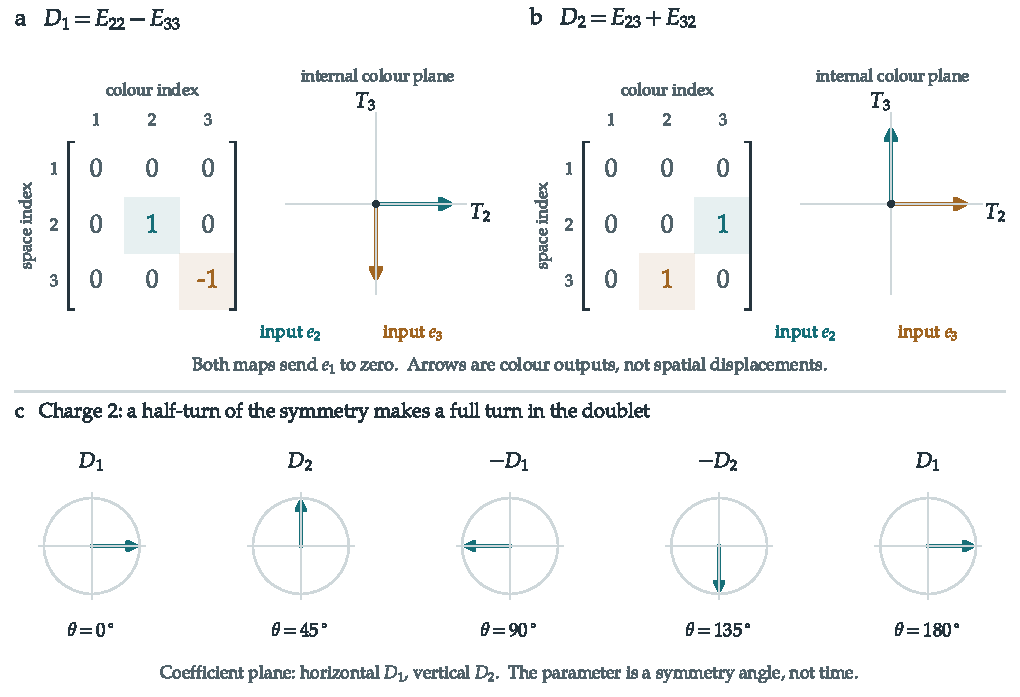
\includegraphics[width=\linewidth]{figures/helike-doublet.pdf}
\caption{\textbf{Helike's actual homogeneous doublet in the convention of \S4.}
$D_1=E_{22}-E_{33}$ and $D_2=E_{23}+E_{32}$, with $E_{ka}$ equal to one in row $k$, column $a$, and zero elsewhere.
Rows are spatial inputs $e_k$; columns are internal colour components $T_a$.
The arrows show $b_D(e_k)=\sum_a D_{ka}T_a$: teal for input $e_2$, gold for input $e_3$.
They lie in the colour plane, not the spatial tangent plane. Both maps annihilate $e_1$.
Below, $R_\theta$ rotates $e_2$ toward $e_3$ (and $T_2$ toward $T_3$), giving
$R_\theta D_1R_\theta^T=\cos(2\theta)D_1+\sin(2\theta)D_2$.
The two complex combinations have charges $\pm2$; the plot uses the real pair.
The matrices are unnormalized, each with Frobenius norm $\sqrt2$; divide by $\sqrt2$ for unit matrix norm.
This shows the homogeneous member, not the higher-harmonic family or a global $L^2$ normalization.}
\label{fig:helike-doublet}
\end{figure}

\clearpage
\subsection*{The proposed mechanism}

\textbf{The theory.} Topology organizes the field's possible routes; geometry and kinetic energy give them their costs;
quantum dynamics determines the lowest excitation. I propose that the mass gap is the lowest note of this combined
structure, carried by a shape that leans toward a winding-changing route. The fine grain dresses that shape, and the
note is inherited all the way out to infinite space. If the theory is true, it says five things.
\begin{enumerate}
\item \textbf{The gap has a name:} in a small room it is carried by Helike, a twisting shape of charge~2 under the room's rotation symmetry, or by
her competitor, a breathing shape of charge~0, and as the room grows the carrier changes only at exact, countable
switches (\S4--5). \item \textbf{The landscape gives the carriers their costs:} the reduced potential is the squared slope
of Chern--Simons, measured with the field-space metric. The competitor follows the one downhill direction of
Chern--Simons at the winding-one vacuum: the field's first step toward the other winding vacuum. The quantum ordering
comes from the potential and kinetic energy together. This suggests a mechanism for the scalar glueball being
lightest (\S5). \item \textbf{Tensor-like and scalar-like channels trade places at a
calculable point,} $s_0^*(t)=(t+2)(\sqrt{t+8}-\sqrt t)/(4\sqrt t)$, which is $1.1436$ at $t=3$ at harmonic order; the switches registered at stronger coupling rise from it (\S5). \item \textbf{The
fine grain cannot erase the note:} the computed logarithmic divergence has the asymptotically free coefficient
$b_0=22/3$; finite and kinetic dressing must still be controlled (\S6). \item \textbf{The infinite world is the last room:} infinite
space is the end of a family of spheres, and the gap in units of the theory's scale stays uniformly above zero,
including at that end (\S7--8).

\end{enumerate}
Simulations provide evidence for a gap and scalar glueball ordering; perturbation theory establishes asymptotic freedom,
not the nonperturbative gap. My proposal is to connect those observations through one geometric mechanism.


The central conjecture is stated after the geometric definitions in \S2. I retain the standing of each supporting
statement beside it; Appendix~\ref{app:register} collects the complete status and coverage maps.

\subsection*{The problem, as it is posed}

The target is not mine. It is the Millennium Prize problem as Jaffe and Witten wrote it~\cite{JaffeWitten}. For every
compact simple gauge group $G$ (the symmetry group of the field, such as $SU(2)$ or $SU(3)$), construct quantum
Yang--Mills theory on four-dimensional space-time $\mathbb R^4$ and show two things. First, it exists as a genuine
quantum field theory: it satisfies axioms at least as strong as Wightman's~\cite{StreaterWightman}, or in Euclidean form
those of Osterwalder and Schrader~\cite{OS73,OS75} (Euclidean invariance, reflection positivity, regularity, clustering),
from which a relativistic theory is reconstructed; it has local field operators for the gauge-invariant polynomials in
the curvature $F$, such as $\mathrm{tr}\,F^2$; at short distance it agrees with perturbation theory and asymptotic
freedom~\cite{GrossWilczek73,Politzer73}; and it is non-trivial, not a free field in disguise. Second, it has a mass gap:
the spectrum above the vacuum begins at a strictly positive, finite energy. Normalized states
orthogonal to the vacuum have energy expectation at least $\Delta>0$; a superposition with a vacuum component need not.

The problem is hard because of two infinities. The \emph{ultraviolet} is the fine grain: zoom in and the field has ever
finer ripples, infinitely many, which must be controlled together (renormalization). The \emph{infrared} is the growing
room: zoom out, and the gap must survive in infinite space, exactly where the coupling becomes strong and no small
parameter is left. Every computation, mine included, cuts off one or both, with a lattice of spacing $a$ or a room of
finite size. The difficulty is to remove the scaffolding and keep the answer.

\begin{claim}{OPEN}{The Clay target}\label{b:clay}
For $G=SU(2)$, and then every compact simple $G$, quantum Yang--Mills theory on $\mathbb R^4$ exists with every
property above (OS and so Wightman axioms, local fields, short-distance agreement, non-triviality, a unique vacuum), and
its Hamiltonian has nothing in $(0,\Delta)$, with a nonempty excitation spectrum and finite first spectral threshold
$m\ge\Delta=c\,\Lambda>0$. Here $\Lambda$ is an energy scale in a fixed renormalization scheme,
and $c>0$ a dimensionless number. I work at vacuum angle $\theta=0$.
\evidence{The problem itself~\cite{JaffeWitten}. My register splits it into 29 lines and maps every clause to them
(Table~\ref{tab:clay}); it rests on four hypotheses, H3, H4$'$, H6, H7~\cite{ClosedSet}.}
\lines{1--29}
\end{claim}

\subsection*{Relation to earlier work}

What has been done shows where the wall is. Interacting theories were built in two and three
dimensions~\cite{GlimmJaffe}; two-dimensional Yang--Mills is solved exactly~\cite{Migdal75,GrossWitten80,Sengupta97,Levy03};
on a lattice at strong coupling the gap is a theorem~\cite{OsterwalderSeiler78,ShenZhuZhu23}, at the wrong end of the
coupling. In four dimensions Ba{\l}aban
controlled the ultraviolet in a finite box~\cite{Balaban}, and Magnen, Rivasseau and S\'en\'eor built the $SU(2)$
Schwinger functions with an infrared cutoff kept~\cite{MRS93}. Nobody has removed the infrared cutoff. Physically the
gap is not in doubt: simulations find a lightest glueball, a scalar $0^{++}$~\cite{MorningstarPeardon99}.

Simulations show a gap with the scalar lightest~\cite{MorningstarPeardon99};
perturbation theory shows asymptotic freedom~\cite{GrossWilczek73,Politzer73}; strong-coupling expansions prove a gap at
the strong-coupling end~\cite{OsterwalderSeiler78}. My theory proposes a geometric connection between them:
topology organizes the landscape's routes; its geometry makes the downhill Chern--Simons direction locally soft;
quantum dynamics combines that landscape with kinetic energy, and the fine grain dresses the resulting carrier.
In this picture they are parts of one mechanism: the
lowest note of the folded space of field shapes, named in the small room and followed to infinite space. The finite-volume road
is L\"uscher's and van Baal's~\cite{Luscher83,KollerVanBaal88,vanBaal00}; the stretched sphere, the identified floor, the
named carrier, the sources, the harmonic switch and the proposed inheritance along scale are the route developed here.

The scale $\Lambda$ is where the problem turns geometric. The classical equations contain no length; the quantum theory
makes an energy scale through the running coupling; in units $\hbar=c=1$, $1/\Lambda$ is the associated length.
A gap that is a pure number times that energy scale is a
property of shape, not of any box. So I begin with the shape.

% s2: begin with the geometry. ASCII only.
\section*{2. Begin with the geometry}

I start from the geometry the theory already lives on, a principal fibre bundle, equipped with a connection and a
space-time metric. The \emph{base} is space-time (or a spatial slice in the Hamiltonian picture).
Locally its fibres are copies of the \emph{structure group} $SU(2)$, with no preferred group identity in each fibre.
Its double cover of $SO(3)$ concerns internal colour rotations, not space-time spin. Its centre $\{\pm1\}$ permits
half-integer colour representations and distinguishes fundamental from adjoint loops; it does not alone prove
confinement~\cite{tHooft78}. A \emph{connection} $A$ is the gauge field, a rule for
carrying the fibre along a path; around a closed loop $C$ it returns a \emph{holonomy} $\mathrm{Hol}_C(A)\in SU(2)$, and
its infinitesimal holonomy is the curvature $F$. A \emph{gauge transformation} relabels each fibre, so the physical
configurations are connections modulo relabelling, the space $\mathcal A/\mathcal G$. That space is curved and folded,
and no single choice of labels covers it (the Gribov problem~\cite{Gribov78,Singer78}). It has \emph{topology}: winding
classes of large gauge transformations $\pi_3(SU(2))=\mathbb Z$. Chern--Simons shifts by that integer; on general
connections it is continuous, not an integer-valued topological label~\cite{ChernSimons74}. Vacuum representatives are joined by
instantons~\cite{BPST75,JackiwRebbi76,CallanDashenGross76}. The quantum theory adds a measure, a spectrum, and a sorting of
modes into slow and fast.

\textbf{Three things working together.} I do not ask topology to assign an energy by itself. It describes the global
connections and identifications of the space of physical fields. The spatial metric and the Yang--Mills action give
that space its ruler and its magnetic-energy landscape. The kinetic term measures the energy cost of variation of a
wavefunctional across field configurations. Quantum dynamics combines them, with the gauge constraints, to determine
the vacuum and the excitations~\cite{KogutSusskind75,vanBaal00}. These are aspects of the same theory, not three extra
forces. The same topology can carry different geometries and different spectra. I want to follow what changes in
the field, not only the number attached to that change. Van Baal describes how wavefunctionals spreading across
identified boundaries of configuration space become sensitive to its topology~\cite{vanBaal92Topology}; that is a
physical connection between the global shape of the space and its low energies.

A connection component at a point depends on the gauge; local invariant quantities such as $\mathrm{tr}\,F^2$ do not.
Loops give another set of physical readings:
$W_C=\mathrm{tr}_\rho\,\mathrm{Hol}_C(A)$ is unchanged by relabelling, because the trace does not see conjugation, and
the complete compatible loop data reconstruct a smooth connection up to gauge under the hypotheses of
Giles' theorem~\cite{Giles81}. A finite set of measured loops is not that complete data. Wilson's lattice theory~\cite{Wilson74} is this
bundle sampled: the base at the vertices of a grid of spacing $a$, a group element $U_\ell$ on each edge, and the action
read from the holonomy $U_p$ of each elementary square (plaquette).

\begin{claim}{PROVED}{The lattice measure lives on connections modulo gauge}\label{b:wilson}
$d\mu_{a,L}=Z^{-1}\exp\bigl(-\beta\sum_p(1-\tfrac12\mathrm{tr}\,U_p)\bigr)\prod_\ell dU_\ell$, $\beta=4/g^2$, is gauge
invariant and descends to a probability measure on lattice connections modulo gauge. No gauge fixing is needed for
these integrals; this avoids, rather than solves, the Gribov gauge-fixing obstruction. Every Wilson loop is gauge invariant.
\evidence{Traces of holonomies and an invariant Haar measure~\cite{Wilson74}; checked in my engine (\S3).}
\lines{1}
\end{claim}

\begin{claim}{PROVED (CITED)}{Reflection positivity and the transfer matrix}\label{b:rp}
The Wilson measure is reflection positive, so there are a Hilbert space, a vacuum and a transfer matrix $T=e^{-aH}$ with
$H\ge0$.
\evidence{Osterwalder and Seiler~\cite{OsterwalderSeiler78}, in the sense of~\cite{OS73,OS75}.}
\lines{2}
\end{claim}

Two choices shape the rest. The size of the room is a coordinate of a separate parameter space, not a nuisance, so the gap is a function
over the family of rooms (\S7). The physical base is not being identified with this parameter space.
The rooms are spheres throughout; I retain homogeneous fields as a slow sector with topological information,
without assuming they exhaust the low-energy physical states. Infinite space is the proposed end of the family (\S8). First, the lattice
already gives the gap a meaning at strong coupling, where it can be read off by hand.

% s3: the note of one turn (strong coupling). ASCII only.
\section*{3. The note of one turn}

Everything physical about a gauge field is carried by its turns: carry a frame around a loop and see how far it comes
back rotated. In the purely electric strong-coupling limit the first excitation is the
smallest closed flux loop. Wilson's plaquette term $1-\tfrac12\mathrm{tr}\,U_p=1-\cos\alpha$
is half the \emph{squared} chord distance between the unit quaternions $U_p$ and $1$; in \emph{Three Ways Across a Turn}~\cite{ThreeWays}
I compare it with the arc and the tangent. The cleanest view is the Hamiltonian lattice of Kogut and
Susskind~\cite{KogutSusskind75}: continuous time, a cubic spatial lattice, and at strong coupling an energy that is
\emph{electric}, $g^2/(2a)$ times the quadratic Casimir $C_2$ on each link. The Casimir is the Laplacian of the group,
and $SU(2)$ is a three-sphere, a closed curved shape with a lowest nonzero note: $C_2(j)=j(j+1)$, smallest at
$C_2(\tfrac12)=\tfrac34$, which exists only because $SU(2)$ double covers $SO(3)$ (on $SO(3)$ alone it would be $2$).
Gauss's law allows electric flux only in closed loops, and the shortest is one plaquette.

\begin{claim}{PROVED}{The electric gap is one turn}\label{b:electric}
On the cubic lattice (infinite, or periodic with side $L\ge4$) with no external charges, $H_E=(g^2/2a)\sum_\ell C_2(\ell)$
has a unique ground state of energy $0$ and first excited level exactly $4\cdot\tfrac{g^2}{2a}\cdot\tfrac34=3g^2/(2a)$:
one plaquette loop in spin $\tfrac12$.
\evidence{Peter--Weyl splits gauge-invariant states by link spins; excited links must form cycles of at least four edges
\cite{KogutSusskind75,HelikeReport}.}
\lines{4}
\end{claim}

The magnetic term, of order $1/(ag^2)$, mixes in other configurations, so $3g^2/(2a)$ is the leading term of the gap. Two
lattices must be kept apart here (I once mixed them; the register records the correction~\cite{ClosedSet}). On the
\emph{Euclidean} lattice, with discrete time, a strong-coupling gap is a theorem; on a fixed finite
\emph{Hamiltonian} lattice the leading value follows by perturbation.

\begin{claim}{PROVED (CITED)}{A gap at strong coupling}\label{b:strong}
For small $\beta$ the cluster expansion converges and truncated correlations of local gauge-invariant observables decay as
$e^{-m(\beta)\cdot\text{distance}}$, $m(\beta)>0$; by reflection positivity this is a gap of the transfer matrix.
\evidence{Osterwalder and Seiler~\cite{OsterwalderSeiler78}; by another road, Shen, Zhu and Zhu~\cite{ShenZhuZhu23}.}
\lines{3}
\end{claim}

\begin{claim}{PROVED}{The leading Hamiltonian gap (by deduction)}\label{b:kato}
On a finite Hamiltonian lattice the magnetic term is a bounded perturbation of $H_E$, so the full Kogut--Susskind gap is
$3g^2/(2a)+O_L(1/(ag^2))$ as $g\to\infty$. The constant here may depend on lattice size $L$.
\evidence{Kato's analytic perturbation theory~\cite{Kato}. A volume-uniform Hamiltonian statement needs a separate
uniform argument; the Euclidean result in Box~\ref{b:strong} is not by itself that argument.}
\lines{5}
\end{claim}

In two dimensions the whole story is exact at every coupling: in a tree gauge the plaquettes are independent and every
loop factorises~\cite{Migdal75,GrossWitten80}.

\begin{claim}{PROVED}{Two dimensions: each loop's area law is its Casimir}\label{b:2d}
For $SU(2)$ on a planar lattice, a simple loop around $|A|$ plaquettes has $\langle\chi_j\rangle/d_j=(I_{2j+1}(\beta)/
I_1(\beta))^{|A|}$, so $\sigma_j=2C_2(j)/\beta+O(\beta^{-2})$ in lattice area units and $\sigma_1/\sigma_{1/2}\to8/3$. A centre vortex (links
crossed by a sheet multiplied by $-1$) multiplies a spin-$j$ loop by $(-1)^{2jn}$, $n$ its winding around the vortex:
half-integer loops feel it, integer loops do not.
\evidence{Character factorisation~\cite{Migdal75,GrossWitten80}; $\chi_j(-U)=(-1)^{2j}\chi_j(U)$, the centre-vortex
picture~\cite{tHooft78,Greensite03}. Casimir scaling is seen in four dimensions~\cite{Bali00}.}
\lines{6}
\end{claim}

I checked the two-dimensional loop identities in GIGI, my database engine, with the lattice connection stored as a bundle and every loop read
only by point queries: the loops match the character formula within $2\sigma$, a random gauge rewrite changes no loop by
more than $1.23\times10^{-15}$, and a planted vortex flips the fundamental loop exactly and leaves the adjoint
alone~\cite{HelikeReport}.

Strong coupling gives the note but not the continuum, and it is never an end of the family of rooms, since every
room's continuum limit sends the bare coupling to zero (\S7). Two dimensions has an exact area law but no propagating
gluons. Near the identity the Wilson plaquette cost is quadratic in angle, with a coupling-dependent coefficient;
that local cost alone does not determine a quantum gap. So in
four dimensions the note has to be found again, carried by a shape, in a room small enough that the coupling is weak.

% s4: the small room. ASCII only.
\section*{4. The small room}

Asymptotic freedom makes small rooms weakly coupled: on a space of size $R$ the effective coupling $g^2(R)$ goes to zero
as $R$ shrinks~\cite{GrossWilczek73,Politzer73}. So a small closed space is where the field can be solved, the finite-volume programme of L\"uscher on the torus~\cite{Luscher83}, of Koller and
van Baal~\cite{KollerVanBaal88}, and of van Baal and van den Heuvel on the three-sphere~\cite{vanBaalvandenHeuvel94,vanBaal00}.

\textbf{The room and its slowest modes.} The three-sphere is the group $SU(2)$, with three left-invariant directions
$\sigma^1,\sigma^2,\sigma^3$. The Berger sphere $S^3_t$ has metric $t(\sigma^1)^2+(\sigma^2)^2+(\sigma^3)^2$: round at
$t=1$, stretched along the circles of $\sigma^1$ otherwise; my controls use $t=3$. Stretching leaves one circle of
rotations, and its integer charge $m$ labels states as spin does on the round sphere. The slowest fields are the
homogeneous ones, $A=q_{ka}\theta^kT_a$, with $\theta^k$ the orthonormal coframe and $q$ a constant $3\times3$ matrix
(rows: space; columns: colour). The only gauge transformations that keep a field homogeneous are constant colour rotations.

\begin{claim}{PROVED}{The slow space}\label{b:slow}
Homogeneous fields modulo gauge form $\mathbb R^9/SO(3)$, $q\mapsto qO^T$. With $q=PO$, $P$ symmetric with eigenvalues
$\lambda_i$, the flat measure is $\prod_{i<j}|\lambda_i+\lambda_j|\,dP\,dO$: the finite version of the weight of
$\mathcal A/\mathcal G$.
\evidence{Residual gauge group and polar Jacobian~\cite{HelikeReport}; the quotient picture of~\cite{Singer78,Gribov78}.}
\lines{7}
\end{claim}

The quotient has a fold: the colour-blind shape $qq^T$ does not see the sign of $\det q$, so the slow space is a drum
folded over on itself, two sheets glued where $q$ loses rank. The physical operator crosses the fold freely (the
\emph{natural} realization); a basis that vanishes there sees a wall (the \emph{Dirichlet} realization).

\textbf{The line between two windings.} On $S^3=SU(2)$ the Maurer--Cartan form $x^{-1}dx$ is a flat connection of winding
one, gauge equivalent to $A=0$, and it is homogeneous: the point $q_{\rm MC}=\mathrm{diag}(t^{-1/2},1,1)/g$. The line
$\lambda q_{\rm MC}$ joins winding zero to winding one, the finite image of the vacuum periodicity of Jackiw--Rebbi and
Callan--Dashen--Gross~\cite{JackiwRebbi76,CallanDashenGross76}.

\begin{claim}{PROVED}{Topology on the Maurer--Cartan line}\label{b:mc}
Along the line $CS(\lambda)=3\lambda^2-2\lambda^3$ and $V=(1+2/t)(\lambda-\lambda^2)^2/(2g^2)$: a double well with zeros
at the two windings and the sphaleron at $\lambda=CS=\tfrac12$. My controls hold the background $q_{\rm bg}=s\,q_{\rm MC}$
just past the winding-one vacuum, with sources that vanish at $s=1$.
\evidence{$d\Omega=-\Omega^2$ and a diagonal computation, confirmed to $10^{-13}$~\cite{HelikeReport,ClosedSet}; the
sphaleron is the finite analogue of Klinkhamer--Manton's~\cite{KlinkhamerManton84}.}
\lines{8}
\end{claim}

The sources are my own departure. They live in the reduced model only, with no gauge-invariant lift yet, and they are
scaffolding that \S5 removes.

\begin{claim}{PROVED}{Theorem A: the spectrum is discrete}\label{b:thmA}
For $t\ge1$ and $0<s<(t+2)/(t+1)$, $V\ge\tfrac\kappa2\|q\|^2-S^4/(2g^2)$ with $\kappa>0$ and $S=\sqrt t+2/\sqrt t$. The
reduced Hamiltonian is essentially self-adjoint with compact resolvent: its spectrum is discrete in every charge sector.
\evidence{Expand the square, bound $\|\mathrm{cof}\,q\|^2\ge3|\det q|^{4/3}$, then~\cite{ReedSimonIV}.}
\lines{9}
\end{claim}

\textbf{Helike and her competitor.}\ \spine{1} The lowest note in the room has a name. Helike is the charge-2 field
$(\hat\theta^1+i\hat\theta^2)\otimes(\tau_1+i\tau_2)$: frame and colour turn together, at the largest charge the circle
allows. Her competitor is the charge-0 \emph{breathing} mode in the plane $\mathrm{diag}(x,y,y)$, which \S5 shows is the
direction of topology.

\begin{claim}{PROVED (CITED)}{Helike is an exact eigenvector and the floor}\label{b:helike}
For every $t$, every circle-symmetric homogeneous background $(x,y)$ and every harmonic $j$, Helike is an exact
gauge-orthogonal eigenvector of the Yang--Mills Hessian, alone in her charge block, with eigenvalue
$(x+(j+2)/\sqrt t)^2+2\sqrt t\,x-y^2$ (helicity squared minus the flux along her circle), and she is the floor of the
spectrum for $t\in[2.75,10]$ on the stated domain. In the reduced model $\omega_H^2=2s(1+2/t-s)$.
\evidence{My papers \emph{By Enough, But Not Too Much} and the Floor Theorem v3.3~\cite{ByEnough,Floor}, not yet
refereed; the reduced formula in~\cite{HelikeReport}.}
\lines{10}
\end{claim}

At the controls ($t=3$, $s=1.15$) the two are close, $\omega_H=1.0901$ against $\omega_C=1.1067$. Ordering the true
quantum levels needs a count: in charge 0, no third level may hide below a threshold $\rho_C$.

\begin{claim}{CONJECTURE}{H1 ($S_C$): at most two charge-0 levels below $\rho_C$}\label{b:sc}
At each control, the natural realization has at most two charge-0 colour-singlet eigenvalues below
$\rho_C=E_0^c+2\omega_H-\omega_{\min}/4$.
\evidence{The route is proved in 128-bit ball arithmetic except the last Lehmann step~\cite{Lehmann}, whose margins
($+0.21$ to $+0.24$) are floating point; the interval version (R2) remains.}
\lines{11}
\end{claim}

\begin{claim}{CONDITIONAL}{Helike lowest at the controls (on H1)}\label{b:order}
At $t=3$, $s=1.15$, Helike's level lies strictly below the second charge-0 level for three of four certificates
$(g^2,M_q)$, covering $g^2=0.002$ and $0.004$, with margins $+0.0072$, $+0.0100$, $+0.0121$; the fourth, $(0.004,6)$, is
unresolved. A reduced-model statement.
\evidence{Min--max and Kato--Temple bounds~\cite{Kato49} with outward rounding; every verdict matched a prediction
registered in advance~\cite{HelikeReport}.}
\lines{12}
\end{claim}

\begin{claim}{CONJECTURE}{The fold costs only tunnelling}\label{b:fold}
For each level $k$, $0\le\lambda_k(H_D)-\lambda_k(H)\le C_{k,\epsilon}e^{-2(d_0-\epsilon)/g^2}$, $d_0$ the Agmon distance
to the fold.
\evidence{Proved: the fold is classically forbidden and natural levels lie below Dirichlet ones. The rest is the
semiclassics of~\cite{Agmon82,Simon83}. Since $\det q$ is the Chern--Simons cubic, fold and winding are one odd term.}
\lines{9, 11}
\end{claim}

So with the sources on, Helike is lowest; \S5 shows that with them off the competitor is, and asks why, and where they
trade places.

% s5: who carries the note (points 1-3 of the theory). ASCII only.
\section*{5. Who carries the note}

The Hamiltonian commutes with the room's circle of symmetry, so it never mixes charges. Helike has charge $\pm2$ (the
$m=\pm2$ part of a spin-2, tensor-like object); her competitor has charge 0 (scalar-like).

\begin{claim}{PROVED}{Different charges cross exactly}\label{b:cross}
Helike and the competitor lie in different invariant sectors of the Berger circle, so their levels cross exactly and the
carrier is well defined on each side of a crossing.
\evidence{The circle commutes with the Hamiltonian at every $s$ and $g$; analytic perturbation theory per
sector~\cite{Kato}.}
\lines{17}
\end{claim}

\spine{2} Topology decides who is lightest. With the sources off, the potential of the room is the squared slope of
one function, the Chern--Simons number: Witten's form of a Schr\"odinger operator~\cite{Witten82}, whose low levels sit
at the critical points of that function, sorted by their number of downhill directions.

\begin{claim}{PROVED}{The landscape is the slope of Chern--Simons; the competitor is the topological direction}\label{b:susy}
Let $\omega=(\sqrt t,t^{-1/2},t^{-1/2})$, $S=\sum_k\omega_k$ and $W(q)=\tfrac12\sum_k\omega_k\|q_k\|^2-g\det q$. Then
$V_0=\tfrac12|\nabla W|^2$, $W=CS/(2\sqrt t\,g^2)$ on homogeneous fields, and $H=\tfrac12\sum_ia_i^*a_i+\tfrac32S$
exactly, $a_i=\partial_i+\partial_iW$; so the vacuum energy is $\tfrac32S$ up to exponentially small terms. Zero field is
the minimum of $W$; $q_{\rm MC}$ is a saddle of $W$ with one downhill direction, and that direction is the competitor,
pointing back along the path toward the other winding vacuum. Its frequency
$\omega_C=\tfrac12(\sqrt{t+8}-\sqrt t)$ ($0.7923$ at $t=3$) lies below Helike's $\omega_H=2/\sqrt t$ ($1.1547$) and every
other mode, for every $t>0$.
\evidence{$\partial\det q/\partial q_{kc}=\mathrm{cof}(q)_{kc}$ and exact block diagonalization of the Hessian, confirmed
by the referee pass~\cite{ClosedSet,Witten82}. Proved for the undressed reduced operator at $s=1$.}
\lines{8, 18}
\end{claim}

If I could put only one claim first it would be this: the cheapest way to excite the unsourced room is to lean toward
changing its topology. If it survives into the full theory, it is why the scalar glueball is lightest, which simulations
see~\cite{MorningstarPeardon99} and nobody has explained.

\spine{3} Tensor and scalar trade places at a calculable point. Turn the sources on ($s>1$): Helike's frequency
$\omega_H(s)^2=2s(1+2/t-s)$ falls toward the competitor's, and the order reverses.

\begin{claim}{PROVED}{The harmonic switch}\label{b:switch0}
At harmonic order the tensor (charge $\pm2$) and scalar (charge 0) carriers trade places at
$s_0^*(t)=(t+2)(\sqrt{t+8}-\sqrt t)/(4\sqrt t)$, which is $(5\sqrt{33}-15)/12=1.1436$ at $t=3$ and lies inside Theorem
A's window exactly when $t>1$.
\evidence{Closed-form root of the charge-0 secular equation~\cite{ClosedSet}.}
\lines{18}
\end{claim}

\begin{claim}{CONJECTURE}{The carrier changes only at the switch}\label{b:switch}
In the reduced model, for $s>s^*$ Helike carries the note and for $s<s^*$ the competitor does; at $s=1$ it is the
competitor. The registered switches $s^*=1.1674$, $1.1809$, $1.1931$ at $g^2=0.03$, $0.05$, $0.07$ rise from $s_0^*$ as
the coupling grows.
\evidence{The rise matches the anharmonic prediction at leading order; the registered values do not include the fast
dressing of \S6~\cite{ClosedSet}.}
\lines{18}
\end{claim}

\begin{claim}{CONDITIONAL}{A switch exists}\label{b:ivt}
At weak coupling ($g^2\lesssim0.0075$, $t=3$), given H8 at $s=1$ and Helike lowest at the controls (Box~\ref{b:order},
on H1), exact crossing and continuity give a switch. At the registered couplings the controls at $s=1.15$ already have the
competitor lowest, so existence there needs one more control at some $s_1\in(s^*,1.25)$ where Helike is lowest.
\evidence{Deduction from lines 12, 17, 19 and H8; the bracketing gap was found by the referee pass~\cite{ClosedSet}.}
\lines{18, 12}
\end{claim}

The sources are scaffolding; the physical room has none, and the bridge back is short.

\begin{claim}{PROVED}{The source bridge $s\to1^+$ (by deduction, reduced model)}\label{b:bridge}
Ordered eigenvalues and spectral projections of the reduced operator are continuous on $[1,s_1]$ for any $s_1$ in the
window.
\evidence{A type-(A) analytic family~\cite{Kato}. Only ordered eigenvalues are continuous through a charge-0 avoided
crossing near $s=1+0.95\,g^2$; this is not a bridge in the full theory~\cite{ClosedSet}.}
\lines{19}
\end{claim}

\textbf{The honest catch.} All of this is about the undressed reduced operator. In full Yang--Mills $q_{\rm MC}$ is a
gauge copy of $q=0$, so the two wells are one point; near $q=0$ the charge-0 and charge-$\pm2$ two-quantum states tie at
$2/\sqrt t$, and the tie is broken at order $g^2$ by a kinetic term of the fast modes (\S6).

\begin{claim}{OPEN}{H8 in the physical theory}\label{b:h8}
At $s=1$ the lowest excitation has charge 0. True for the undressed reduced operator (margin $0.3624$ at $t=3$); in the
physical theory decided only at $O(g^2)$, by the kinetic correction of Box~\ref{b:kinetic}.
\evidence{The register's correction to H8~\cite{ClosedSet}; the next step is a pair of one-sided bounds with constants
summing below $5.18$ at $g^2\le0.07$.}
\lines{18, 16}
\end{claim}

\textbf{Theta and tunnelling.} The degree-one gauge map shifts the Chern--Simons number by one, so the vacuum angle
$\theta$ is a Bloch phase~\cite{JackiwRebbi76,CallanDashenGross76}, and tunnelling between windings is set by the Agmon
distance~\cite{Agmon82,Simon83}.

\begin{claim}{PROVED}{The tunnelling length is pinned by topology}\label{b:agmon}
In variables $q=p/g$ the Agmon distance from zero field to the winding-one orbit satisfies
$1/(2\sqrt t)\le d\le\sqrt{(t+2)(2t+1)}/(6t)$ ($0.2887\le d\le0.3287$ at $t=3$), so tunnelling moves levels by
$O(e^{-2d/g^2})$. The lower bound is Bogomolny's: $\int|\nabla W|\,|dp|\ge\Delta W$.
\evidence{The analogue of the instanton bound $8\pi^2|\Delta CS|/g^2$~\cite{BPST75,tHooft76}; the upper bound is the
straight path~\cite{ClosedSet}.}
\lines{18, 19}
\end{claim}

I conjecture that theta barely moves the note, $|\Delta(\theta)-\Delta(0)|\le C\,e^{-8\pi^2/g^2}$ by tight binding over
the chain of vacua~\cite{tHooft76}; nothing in the theory uses it at $\theta=0$.

If the switch rises with the coupling, and a larger coupling is a larger room, the scalar's territory grows with the room.

\begin{claim}{CONJECTURE}{The small-room order is the glueball order}\label{b:glueball}
$s^*$ keeps rising along the growing room, and the small-room order, charge 0 below charge 2, becomes
$m(0^{++})<m(2^{++})$ in infinite volume.
\evidence{Lattice order~\cite{MorningstarPeardon99}. The rise is first order only, and continuing circle charges to
$J^{PC}$ needs an argument I do not have. I quote no mass ratios.}
\lines{18, 20}
\end{claim}

The carriers are named, topology orders them, and they trade places at a point I can write down, all read from nine
slow numbers. What of the infinitely many fast modes left out?

% s6: the fast modes dress; they do not erase (point 4 of the theory). ASCII only.
\section{The fast modes dress; they do not erase}

\spine{4} The fine grain cannot erase the note. A field on the sphere has infinitely many modes finer than the room. My
answer to what they do to the slow note is that they dress it. The logarithmically divergent part matches the running
of the coupling~\cite{GrossWilczek73,Politzer73}; finite effects remain, and controlling them is part of my conjecture.

\textbf{The scale fibration.} $S^3_t$ is itself a group, so fields on it sort by how they transform under left
translations (Peter--Weyl): sectors $j=0,1,2,\dots$, sector $j$ with multiplicity $j+1$. Sector $j=0$ is exactly the
homogeneous fields. So the configuration space is a fibration: a slow \emph{base} (the nine numbers $q$ modulo colour)
and over each point a \emph{fibre} of fast modes, $j\ge1$, locally in a chosen gauge chart. This is not a global
trivialization of the gauge quotient. Here $j$ is twice the representation spin.

\begin{claim}{PROVED}{The slow base is exactly the reduced model}\label{b:pw}
The classical homogeneous restriction and quadratic fluctuation decomposition recover the unsourced reduced
model, with $\mu_{\rm YM}=4\omega^2_{\rm red}$ and background coordinates $M=2gq$ (not the curvature $F$).
The full interacting quantum Hamiltonian also couples slow modes to fast pairs and higher products: it is not a
direct sum of independent $j$-sector theories. A single fast quantum has nonzero left spin and cannot by itself mix
into a left-invariant slow state.
\evidence{Representation theory on $S^3=SU(2)$; the unit map checked to $2\times10^{-8}$~\cite{HelikeReport,ClosedSet}.}
\lines{13}
\end{claim}

On the round sphere van Baal and van den Heuvel keep eighteen degenerate slow modes, left- and
right-invariant~\cite{vanBaalvandenHeuvel94,vanBaal00}; I put the right-invariant ones in the fibre and stretch the
sphere ($t\ne1$). My split rests not on a frequency gap but on the coupling: every slow--fast coupling carries a factor
$g$, through $M=2gq$ near the vacuum chart. That is unconventional, and H2 below must justify it.

\textbf{Born--Oppenheimer.} Freeze the slow variables at $q$. The fast modes form a harmonic system with ground state
$\Omega(q)$ and zero-point energy $E_0(M)=\tfrac12\sum_n\sqrt{\mu_n(M)}$ in the Yang--Mills spectral convention.
Reduced energies are half these energies. On a simply connected chart with a positive fast spectrum and a
nondegenerate normalized real $\Omega$, its Berry connection vanishes locally; this does not assert a global
trivialization across degeneracies. The slow potential receives $\tfrac12E_0(2gq)$ plus further terms of order $g^2$.
The sum diverges, and the regulator must be a function of the spectrum,
never of the sector label: gauge invariance forces a fast shift of exactly $-2$ between the two vacua at $t=1$; a
sector cutoff gives $-8.67$, a heat trace $-1.99999997$.

\begin{claim}{COMPUTED}{The dressing's divergence is asymptotic freedom}\label{b:b0}
$E_0=-\dfrac{b_0}{8\pi^2}\log(\Lambda_{\rm cut}R)\,S_{\rm cl}+E_0^{\rm fin}$ with $b_0=22/3$, the one-loop coefficient
of $SU(2)$. In the saved round-sphere line comparison, the maximum relative discrepancy across seven non-vacuum
points is $7.95\times10^{-4}$; across the five central points it is $6.66\times10^{-5}$.
These are observed discrepancies, not statistical confidence intervals. The proposed subtraction is running $1/g^2$.
\evidence{Heat trace on the Berger slice spectrum~\cite{HelikeReport}; the coefficient of~\cite{GrossWilczek73,Politzer73}.
Computed, not proved; my first pass had the sign wrong, corrected in the register~\cite{ClosedSet}.}
\lines{14}
\end{claim}

This is the place I find most beautiful: the computed ultraviolet logarithm recognizes the known coupling law.
It does not say that the fine grain acts only through that number. Its finite potential and kinetic terms can still
move the note, and asymptotic freedom alone does not prove that the infrared gap survives.

\textbf{Where the fine grain acts.} The frequency equation of \S5 shows how dressing can work without changing the
topology. For an isolated positive-frequency mode, the first-order change is
\begin{equation}\label{eq:dressing}
 \delta\omega=
 \frac{v^T(\delta K_{\rm pot}-\omega^2\delta G_{\rm kin})v}
      {2\omega\,v^TG_{\rm kin}v}.
\end{equation}
For a degenerate block, first diagonalize the corresponding perturbation within that block~\cite{Kato}.
The potential changes the stiffness; the kinetic metric changes the ruler against which that stiffness is measured.
Both can move the note. At a fixed background in the orthonormal reduced coordinates, the potential correction
$\tfrac12E_0^{\rm fin}(2gq)$ gives $\delta K_{\rm pot}=2g^2\nabla_M^2E_0^{\rm fin}$ and hence
$\delta\omega_k=g^2u_k\cdot\nabla_M^2E_0^{\rm fin}\cdot u_k/\omega_k$ for a unit slow mode $u_k$.
This is the potential contribution below; the formula also shows where a kinetic contribution enters.

\begin{claim}{COMPUTED}{The potential part of the dressing widens Helike's lead}\label{b:widen}
At the controls and $g^2=0.002$ the harmonic separation $0.0165$ between Helike and the competitor becomes $0.0191$ (range
$0.0183$--$0.0200$ over regulator windows); at $g^2=0.004$, $0.0216$. This is the potential part of the $O(g^2)$ shift
only.
\evidence{Curvatures of $E_0^{\rm fin}$ along the two modes, $8.89$ and $10.42$, converged to four
digits under the reported spectral-truncation check at fixed prescription, but with regulator-window spreads
$8.65$--$9.08$ and $10.20$--$10.67$ respectively~\cite{HelikeReport,ClosedSet}.}
\lines{15}
\end{claim}

\begin{claim}{OPEN}{The kinetic correction at the same order}\label{b:kinetic}
A second $O(g^2)$ correction is not computed: the non-adiabatic mass of the fast modes dragged by the slow motion (which
screens) plus the Coulomb term of the fast Gauss law (which anti-screens), entering as $-m^{\rm ren}_{u_ku_k}\omega_k$.
Until the full effective Hamiltonian at this order is controlled, the sign of the change in separation is open,
and so is physical H8 (Statement~\ref{b:h8}). Computing this term is necessary, not alone sufficient to settle both.
\evidence{Identified by the referee pass; recorded as the correction to line 15~\cite{ClosedSet}.}
\lines{15, 16}
\end{claim}

Equation~\eqref{eq:dressing} turns this open term into a threshold. In the second-order effective Hamiltonian the
kinetic matrix is $\delta_{ik}-2m^{\rm ren}_{ik}$, so $\delta G_{\rm kin}=2m^{\rm ren}$ to first order and the kinetic
shift of a unit slow mode is $-\omega_k m^{\rm ren}_{u_ku_k}$. At the sourced controls the Helike doublet and the
competitor are separated; a symmetry-preserving correction is treated in their charge blocks, keeping the doublet
together. This is a local expansion with a positive kinetic matrix. For a smooth gapped fast chart with bounded
derivatives, writing the Born--Huang potential as $\Phi(q)=g^2\phi(2gq)$ gives
$\nabla_q^2\Phi=4g^4\nabla_M^2\phi$. Its leading constant cancels in same-well excitation gaps. That local power
counting does not control offsets between different wells or the uniform removal of the fast cutoff.

\begin{claim}{COMPUTED}{How large the kinetic term must be to reverse the order}\label{b:threshold}
Write $m^{\rm ren}=g^2\tilde m$ in the scheme of line~14 ($\zeta$, $\mu R=1$) and
$\kappa=\omega_C\tilde m_{CC}-\omega_H\tilde m_{HH}$ for the competitor and Helike modes. Here $\kappa$ names the
kinetic difference, not the finite-counterterm parameter used elsewhere. At $t=3$, $s=1.15$, combining the recorded
anharmonic coefficient and local quadratic dressing at the same held background gives the linear estimate
\begin{equation}\label{eq:threshold}
 D_{\rm lin}(g^2)=0.01655+g^2\bigl(-2.208+1.258-\kappa\bigr).
\end{equation}
The coefficient $-2.208$ is the reduced model's own anharmonic shift, consistent with the converged separation
$0.01210$ at $g^2=0.002$; $+1.258$ is the fast potential dressing of Statement~\ref{b:widen}.
Within this estimate and for $g^2>0$, Helike lies below this competitor when
$\kappa<0.01655/g^2-0.950$; equality is a tie, and the opposite inequality reverses the order.
The rounded thresholds are $7.33$ at $g^2=0.002$ and $3.19$ at $g^2=0.004$.
This form also handles $0.950+\kappa\le0$, where division by that quantity would mislead.
There is no remainder bound here: these are thresholds for the linear estimate, not certified finite-coupling orderings.

I can also ask how the switch responds. Write $D_0(s)=\omega_C(s)-\omega_H(s)$, and let $a(s)$, $p(s)$ and
$\kappa(s)$ be the anharmonic, potential and kinetic coefficients of this local estimate. If it extends smoothly
to a simple switch, implicit differentiation gives
\begin{equation}\label{eq:dressedswitch}
 \left.\frac{ds^*}{d(g^2)}\right|_{0}
 =-\frac{a(s_0^*)+p(s_0^*)-\kappa(s_0^*)}{D_0'(s_0^*)},\qquad
 D_0'(s_0^*)\simeq2.569 .
\end{equation}
The coefficients belong at the harmonic root $s_0^*=1.14357$, not at $s=1.15$. Freezing them at that nearby control
instead gives $s^*\approx1.1436+(0.950+\kappa)g^2/2.569$, a useful estimate, not the root's evaluated derivative.
Without the fast terms its slope is about $0.86$: at $g^2=0.03,0.05,0.07$ it predicts $1.1693,1.1865,1.2037$,
compared with the registered reduced-model values $1.1674,1.1809,1.1931$ obtained with varying coefficients.
It captures the direction and leading scale, not those values exactly. In the frozen-coefficient estimate the
dressed switch is lower only if $\kappa<1.258$, by $(1.258-\kappa)g^2/2.569$.
\evidence{The saved harmonic frequencies are $1.106657$ and $1.090107$; the potential coefficient is the central
value of the calculation in Statement~\ref{b:widen}, not an uncertainty bound. I have not included displacement
of the equilibrium by the fast force; at fixed sources that can also change the stiffness at $O(g^2)$.
The full matched effective Hamiltonian, a source prescription and remainder control are needed for a physical
switch. The kinetic term remains open.}
\lines{15, 16, 18}
\end{claim}

A script in the repository recomputes every number of this linear estimate from committed receipts
(\texttt{lowest\_note\_threshold.py}).

\begin{claim}{CONJECTURE}{H2 (M3): uniform dressing at small $R$}\label{b:m3}
At $s=1$, on a chart around $q=0$, for $t\ne1$ and small $g(R)$: the levels of the full Hamiltonian (gauge-invariant
spectral cutoff $\Lambda_{\rm cut}$, bare coupling run as above) in a low window converge as $\Lambda_{\rm cut}\to\infty$
and lie within $C\,g^2(R)/R$ of the vacuum-chart reduced levels, uniformly in $\Lambda_{\rm cut}$.
The comparison includes multiplicities and exclusion of extra low states outside the retained sector.
\evidence{Proved pieces: the split, the flat Berry connection, the selection rule. Computed: $b_0$. Templates:
L\"uscher~\cite{Luscher83}, Koller--van Baal~\cite{KollerVanBaal88}, van Baal on $S^3$~\cite{vanBaal00}; rigorous
Born--Oppenheimer for finitely many fast modes with a gap~\cite{Teufel03}.}
\lines{16}
\end{claim}

The route I see is Ba{\l}aban's multiscale method~\cite{Balaban} in Hamiltonian form: integrate the fast modes in
spectral shells; by asymptotic freedom shell $m$ has coupling $g_m=g(2^{-m}R)\le g(R)$, and if each contributes at most
$Kg_m^22^{-m}/R$ after the running of $1/g^2$ (and of a speed of light $c_0$) is subtracted, the sum is geometric and at
most a constant multiple of $g^2(R)/R$. The first step is kinetic consistency, that electric and magnetic couplings run alike, which is
related to Khriplovich's Coulomb-gauge decomposition of $b_0$~\cite{Khriplovich69} and Statement~\ref{b:kinetic}. Granting
H2, well-separated low levels can be compared. An $O(g^2)$ error cannot order channels split only at $O(g^2)$;
that needs H2b's stronger remainder and the physical vacuum chart, not the sourced two-well identification.
But a small room is not the world; the room must now grow.

% s7: the room grows (point 5, first half). ASCII only.
\section{The room grows}

\spine{5} The infinite world is the last room. The radius $R$ belongs to the parameter space of the family. Over each $R$ sits the
whole quantum theory in that room, with its carriers and its gap $\Delta(R)$, the lowest energy above the vacuum over the
entire vacuum-orthogonal physical Hilbert space (every charge, every parity). Changing the renormalization scale
to $1/R$ follows the running coupling, but changing $R$ also changes the physical geometry. These are related, not
identical operations. Asymptotic freedom controls small $R$, not a globally monotone strong-coupling law.

\textbf{Dimensional transmutation.} Pure Yang--Mills has no mass in its Lagrangian. The running manufactures one: holding
the theory fixed while the cutoff is removed defines a scale $\Lambda$ (from the coefficients $b_0=22/3$, $b_1=136/3$).
At fixed squashing $t$, group and $\theta=0$, a finite-room mass has the form $\Lambda f(R\Lambda;t)$.
A constant mass ratio belongs to the infinite-volume limit, if it exists; its value uses a fixed scheme for $\Lambda$.

\begin{claim}{PROVED}{The scaling reduction}\label{b:scaling}
Given that each continuum room exists, $H_R\cong R^{-1}\mathcal K(x)$ for a one-parameter family $\mathcal K(x)$ on the
unit sphere, $x=R\Lambda$. With $\delta(x)=R\,\Delta(R)$ the gap of $\mathcal K(x)$, $\Delta(R)/\Lambda=\delta(x)/x$, and
my uniform-gap route asks for $\inf_{x>0}\delta(x)/x>0$. This is stronger than the infinite-volume step alone needs:
a positive liminf along a converging family as $x\to\infty$. Dimensional analysis does not construct the rooms.
\evidence{Exact dimensional analysis; the existence of each room is H4$'$ (\S8)~\cite{ClosedSet}.}
\lines{20, 23}
\end{claim}

So the gap is a \emph{section} over the half-line $x\in(0,\infty)$, a choice of one number over each room, and the
infrared problem is that it cannot approach zero at the infinite end. Pointwise positivity is not enough.
My uniform bound has three parts.
\emph{(1) Continuity along the base.} A change of carrier between different charges is an exact crossing
(Statement~\ref{b:cross}), and the minimum of finitely many isolated continuous low-level curves is continuous, so such a switch never breaks the section; it
only changes who carries it. \emph{(2) No zero in any room:} a discrete spectrum and a single vacuum give $\delta(x)>0$.
With (1), compactness gives a positive minimum on every closed stretch away from the endpoints.

\begin{claim}{CONJECTURE}{Continuity and positivity on every compact stretch}\label{b:compact}
For every $0<x_0<X$, $\min_{[x_0,X]}\delta(x)/x>0$. Sub-conjectures: (i) compact resolvent and a unique ground state
survive the ultraviolet limit in each room; (ii) $\mathcal K(x)$ is norm-resolvent continuous in $x$~\cite{Kato}.
\evidence{Both hold for every lattice regularization (positivity-improving transfer matrix~\cite{OsterwalderSeiler78})
and for the slow sector by Theorem A; the divergence to remove is the one matched in \S6.}
\lines{20, 17, 19}
\end{claim}

\emph{(3) Control at both ends.} As $x\to0$, $g^2(R)\sim8\pi^2/(b_0\log(1/x))\to0$, and, under H2, the low spectrum is the reduced model
dressed, and $\delta(x)=\delta_0+O(g^2)$ with $\delta_0>0$: tiny rooms are enormously gapped in units of $\Lambda$.

\begin{claim}{CONDITIONAL}{The small-room end}\label{b:smallend}
$\delta(x)/x\to\infty$ as $x\to0$, given a positive limiting reduced gap and H2's exclusion of additional low states.
H8 conjectures the charge-0 carrier, but only $\delta_0>0$ is used here; its ordering need not be settled first.
\evidence{Conditional on H2 (Statement~\ref{b:m3}) in a strengthened form (bounds on the high block and the off-diagonal block);
the small-volume picture of~\cite{Luscher83,KollerVanBaal88,vanBaal00} moved to the sphere.}
\lines{16, 18, 20}
\end{claim}

The large end is the wall. Strong coupling is not it (\S3): every room's continuum limit sends the bare coupling to zero.
What the large end needs is a \emph{finite-size criterion}, the statistical-mechanics idea that mixing checked at one
finite scale forces it at every scale~\cite{DobrushinShlosman85,MartinelliOlivieri94}.

\begin{claim}{CONJECTURE}{The large-room end: one-scale mixing (MS)}\label{b:ms}
There are a physical scale $\rho_*$, an integer $L$ and $\alpha<1$ such that, in a 4-cube of side $L\rho_*$ tiled by
blocks of side $\rho_*$, the total influence of the boundary blocks on smoothed gauge-invariant observables of the central
block is at most $\alpha$, uniformly in boundary condition and cutoff. Then correlations decay at rate
$\log(1/\alpha)/(L\rho_*)$ and $\liminf_{x\to\infty}\delta(x)/x>0$.
\evidence{Proved for lattice spin systems~\cite{DobrushinShlosman85,MartinelliOlivieri94} and lattice Yang--Mills at
strong coupling~\cite{ShenZhuZhu23}; no version for gauge fields uniform in the spacing is known to me.}
\lines{20}
\end{claim}

\begin{claim}{CONJECTURE}{H3 (M2): the gap in the field's own scale}\label{b:h3}
There is $c>0$, depending only on the group and on $t\ne1$, with $\Delta(R)/\Lambda\ge c$ for every $R$. The gap is on
the orthogonal complement of the chosen vacuum, so this hypothesis also excludes other zero-energy states.
Route: Statements~\ref{b:scaling}--\ref{b:ms}.
\evidence{Lattice spectroscopy shows a gap that is a fixed multiple of $\Lambda$~\cite{MorningstarPeardon99}; step
scaling tracks the running across volumes~\cite{LWW91}. This is the infrared half of the problem~\cite{JaffeWitten}.}
\lines{20}
\end{claim}

Every room can be gapped and the theory still massless: if $\delta(x)\sim x^p$ with $0<p<1$, then $R\Delta(R)\to\infty$
while $\Delta/\Lambda\to0$, which only the ratio to $\Lambda$ sees. In GIGI I can follow the section room by
room, a switch showing as an exact crossing: evidence, in the spirit of step scaling~\cite{LWW91}, not proof. The rooms, as they grow, must finally become all of
space.

% s8: from the rooms to all of space (point 5, second half). ASCII only.
\section{From the rooms to all of space}

One road builds the theory in finite boxes and then takes their infinite-volume limit. I start from spheres and stay on spheres: I propose to define the theory on $\mathbb R^4$ as
the $R\to\infty$ end of the continuum theories on $S^3_R\times\mathbb R$. Every ball of fixed size in a sphere of radius
$R$ becomes flat as $R$ grows, providing a candidate geometric limit, not convergence of quantum correlations by itself.
A separate box-versus-sphere identification is unnecessary for this chosen route. In my register, line 29 is folded into line 23,
and two hypotheses become one, H4$'$~\cite{ClosedSet}. Clay asks for no box, only a theory on $\mathbb R^4$ with the
Osterwalder--Schrader properties~\cite{JaffeWitten}.

Inside each room the fine grain must still be removed. The templates are Ba{\l}aban's block-spin renormalization
group~\cite{Balaban} and the construction of Magnen, Rivasseau and S\'en\'eor~\cite{MRS93}.

\begin{claim}{PROVED (CITED)}{The ultraviolet limit in a finite box (partial)}\label{b:box}
Four-dimensional lattice Yang--Mills in a finite box is ultraviolet stable uniformly in the spacing, and the $SU(2)$
Schwinger functions exist with the ultraviolet cutoff removed at fixed infrared cutoff.
\evidence{\cite{Balaban,MRS93}. Neither removes the infrared cutoff or proves a gap; on my geometry they are templates
for the sphere, not results on it.}
\lines{21}
\end{claim}

\begin{claim}{PROVED}{Reflection positivity survives limits}\label{b:rplimit}
$\langle\overline{\Theta F}\,F\rangle\ge0$ for observables $F$ on one side of a reflection is a closed condition, so it
holds in every limit of reflection-positive measures in which these expectations converge.
\evidence{A limit of nonnegative numbers is nonnegative~\cite{GlimmJaffe}; the lattice input is Statement~\ref{b:rp}. For flowed
observables, which are not strictly local, an approximation lemma is needed, which I place inside H4$'$.}
\lines{22, 2}
\end{claim}

Two features are new on the sphere. Nothing mixes time with space on $S^3\times\mathbb R$, so $\mathrm{tr}\,F_{0i}^2$
and $\mathrm{tr}\,F_{ij}^2$ renormalize separately and the limit tunes \emph{two} bare parameters, the coupling $g_0$ and a
speed of light $c_0$. And bare Wilson loops diverge with their perimeter in four dimensions, so I measure observables
smoothed by the gradient flow, perturbatively finite at positive flow time after ordinary renormalization
\cite{Luscher10,LuscherWeisz11}. Flow smears in time as well as space, so a bounded flowed loop is not automatically
a time-slice Hilbert-space operator or an admissible reflection-positive observable.

\begin{claim}{CONJECTURE}{H4$'$: the sphere family (line 23, with line 29 merged)}\label{b:h4}
For every $R$ the ultraviolet limit exists on $S^3_R\times\mathbb R$, with the cutoff of H2 removed, $(g_0,c_0)$ tuned,
and Osterwalder--Schrader regularity bounds. As $R\to\infty$ the flowed correlation functions converge on compact regions
to an $\mathbb R^4$ theory with full Euclidean invariance. This hypothesis also includes a controlled local or
reflection-compatible observable algebra, density of its reconstructed states, and uniform bounds through the limits.
Positive-flow data must be connected to that algebra, not substituted for locality. Given these ingredients and
the remaining OS properties (clustering supplied with H3 below), reconstruction gives a Wightman theory~\cite{OS73,OS75,GlimmJaffe}.
\evidence{I have not constructed this family. Support: the box results~\cite{Balaban,MRS93}; the computed agreement
with $b_0$ (Statement~\ref{b:b0}); perturbative positive-flow finiteness~\cite{Luscher10,LuscherWeisz11}; the
flat-limit derivative is a flowed stress-tensor insertion~\cite{Suzuki13}.}
\lines{23, 29}
\end{claim}

\textbf{The gap survives the limit.} For the gap, the step from rooms to space is one clean lemma. By the spectral
theorem, for $v_A=(A-\langle\Omega,A\Omega\rangle)\Omega$, the autocorrelation
$\langle v_A,e^{-\tau H}v_A\rangle=\int_{[0,\infty)}e^{-\tau E}d\nu_A(E)$ has a positive spectral measure.
An atom at zero is not excluded in advance.

\begin{claim}{PROVED}{The spectral lemma}\label{b:lemma}
If $0\le\langle v_A,e^{-\tau H}v_A\rangle\le C_Ae^{-m\tau}$ for all $\tau>0$ and a set of $v_A$ dense in
$\Omega^\perp$, with finite $C_A$, then
$\mathrm{spec}\,H\cap(0,m)=\emptyset$.
\evidence{Weight of $\nu_A$ on $[0,m)$ would decay more slowly than $e^{-m\tau}$; density does the rest~\cite{ReedSimonIV}.}
\lines{28}
\end{claim}

\begin{claim}{CONDITIONAL}{The gap reaches $\mathbb R^4$, with exponential clustering}\label{b:deduce}
For bounded physical operators $A_R$ with uniformly bounded operator norms, H3 gives the bound with rate
$c\Lambda$ and $C_A\le\sup_R\|A_R\|^2$. If H4$'$ identifies their correlations and supplies dense limiting states,
the bound passes to the limit and the spectral lemma gives $\mathrm{spec}\,H\cap(0,c\Lambda)=\emptyset$.
Locality and Euclidean symmetry then give spatial clustering, with decay rates below the gap and appropriate
observable-dependent constants. A classical sup norm of an arbitrary four-dimensionally flowed observable is not
by itself the required operator-norm or density argument.
\evidence{On H3 and H4$'$. The pass to the limit runs along the sphere family and uses only the sphere-side gap, never
the flat-space result it is proving.}
\lines{28, 20, 23}
\end{claim}

\begin{claim}{CONDITIONAL}{A unique vacuum}\label{b:vacuum}
The $\mathbb R^4$ vacuum is unique: the spectral measure of every truncated state has no atom at zero.
\evidence{It follows from the hypothesis of the lemma, $\nu_A(\{0\})=0$, not from its conclusion; in the reduced model it
holds by Perron--Frobenius~\cite{GlimmJaffe,ReedSimonIV}. So it is conditional on exactly what Statement~\ref{b:deduce} is.}
\lines{27, 28}
\end{claim}

\textbf{An idea for the time--space residue.} Round $S^3\times\mathbb R$ is conformally $\mathbb R^4$ minus a point,
and classical Yang--Mills is conformal; the quantum breaking is the trace anomaly, $\propto b_0\,g^2\,\mathrm{tr}\,F^2$
\cite{CDJ77}, whose size is the $b_0$ I matched in \S6.

My conjecture, an idea rather than an argument, is that the separate tuning of $c_0$ is controlled entirely by this
anomaly, so full Euclidean invariance at $R\to\infty$ follows from the conformal map and the matched $b_0$ (cleanest at
$t=1$; $S^3_t$ is not conformally flat, though every fixed ball still flattens).

If H3 and H4$'$ hold, the limit is a relativistic quantum theory on $\mathbb R^4$ with one vacuum and nothing between it
and $c\Lambda$. That is existence and a gap. The Clay statement also asks what the theory contains.

% s9: what the theory contains. ASCII only.
\section{What the theory contains}

Jaffe and Witten ask for local fields for the gauge-invariant polynomials in the curvature, agreement with perturbation
theory at short distance, a theory that is not free, and all of it for every compact simple group~\cite{JaffeWitten}.

\textbf{Local fields.} Traces of products of $F$ and its covariant derivatives are gauge invariant; graded by dimension
($F$ counts 2, each derivative 1), one of the first is $\mathrm{tr}\,F^2$, the action-density scalar, not the energy density $T_{00}$.
A \emph{renormalized local field} is the limit of a lattice transcription (for
$\mathrm{tr}\,F^2$, the six plaquettes at a point) after a finite mixing with fields of equal or lower dimension; its correlations must be tempered distributions
(continuous on Schwartz test functions) obeying the additional growth condition OS0$'$ that reconstruction
needs~\cite{OS75}. Perturbative renormalization is established~\cite{Reisz88,Reisz89}. At positive flow time, flowed
gauge-field observables need no \emph{additional} renormalization after the underlying theory is renormalized.
The local stress tensor requires matching and a small-flow-time limit~\cite{Luscher10,LuscherWeisz11,Suzuki13}. The nearest
complete non-perturbative analogue is the two-dimensional Gross--Neveu model~\cite{GawedzkiKupiainen85,FMRS86}; nothing
comparable is proved in four dimensions.

\begin{claim}{CONJECTURE}{H6: local fields, and agreement with perturbation theory}\label{b:h6}
On the sphere family and its $\mathbb R^4$ end, every gauge-invariant polynomial in $F$ and its covariant derivatives,
$\mathrm{tr}\,F^2$ first, is a renormalized local field (tempered, OS0$'$), with finite mixing and normalization fixed
by a declared prescription and Ward identities, that reconstructs
to a local covariant operator-valued distribution. A conserved stress tensor generates translations, with trace
$\Theta=-\frac{\beta(g)}{2g}[O]$, $\beta(g)=-\frac{b_0}{16\pi^2}g^3+O(g^5)$. Here the Euclidean trace convention
matches the positive running-plaquette coefficient below, and $O=\sum_{a,\mu,\nu}\mathcal F^a_{\mu\nu}\mathcal F^a_{\mu\nu}$
uses canonically normalized fields with Lagrangian $O/4$. This fixes the sign and normalization instead of silently
identifying $O$ with a differently normalized matrix trace. Vacuum subtraction is understood. At short distance every
correlation function agrees with renormalized perturbation theory in the running coupling, asymptotically to all orders.
\evidence{The perturbative ingredients are established~\cite{GrossWilczek73,Politzer73,ACD77,CDJ77,Luscher10,LuscherWeisz11,Suzuki13};
my sphere coefficient $b_0/8\pi^2$ (Statement~\ref{b:b0}) is the logarithm whose cutoff derivative is the one-loop trace
anomaly~\cite{ClosedSet}.}
\lines{25, 14}
\end{claim}

On the lattice there is an exact starting point for the trace anomaly: varying the inverse coupling in the Wilson measure
differentiates every expectation by minus its correlation with the action, and along the line of constant physics that
derivative is the response to a change of scale.

\begin{claim}{PROVED}{The running-plaquette insertion (lattice identity)}\label{b:anomaly}
On every finite lattice, for parameter-independent $X$, $\partial_{(4/g_0^2)}\langle X\rangle=-\langle X;S_W\rangle$,
$S_W=\sum_p(1-\tfrac12\mathrm{tr}\,U_p)$.
Along the line of constant physics this makes the anomaly density $\Theta_a(x)=-\frac{d(4/g_0^2)}{d\ln a}a^{-4}
\sum_{p\text{ based at }x}(s_p-\langle s_p\rangle)$, with six positively oriented plaquettes per site and
$-\frac{d(4/g_0^2)}{d\ln a}=\frac{b_0}{2\pi^2}+O(g_0^2)$ at one loop. Since
$\sum_{p\text{ based at }x}s_p=a^4g_0^2O/16+\cdots$, the coefficient agrees with $-\beta(g)O/(2g)$.
The exact identity fixes an integrated insertion, not all local contact terms or matching. Its continuum
identification as the stress-tensor trace belongs to H6.
\evidence{Differentiation under the integral; factor and plaquette count verified by the referee pass~\cite{ClosedSet}.}
\lines{1, 25}
\end{claim}

\textbf{Non-triviality.} A free massive theory also has a gap. My first criterion (a nonzero connected four-point function of
$\mathrm{tr}\,F^2$) holds in free theories too, and I withdrew it~\cite{ClosedSet}. The fingerprint I now seek is logarithmic
running: by H6, $|x|^8\langle\Theta(x)\Theta(0)\rangle\sim C_O(N^2-1)/\bigl(16\ln^2(1/|x|\Lambda)\bigr)$ as
$|x|\to0$, an inverse square logarithm, unlike a nonzero dimension-four Wick polynomial in finitely many canonical
free fields with a nonvanishing leading scaling term. A \emph{generalized free field}, Gaussian with an arbitrary
two-point function, could still mimic that two-point fingerprint.

I expected the leading three-point function to distinguish it. That particular prediction is now settled against
me: the free Wick triangle is $T_O=0$ at distinct points in Euclidean four-space. The covariance exchanges the
self-dual and anti-self-dual halves of a two-form. Three exchanges cannot close within either half, so their
trace vanishes. This is an exact geometric cancellation, not a numerical near-zero. It says nothing about
contact terms or the higher-order interacting three-point function.

Four exchanges can return to their starting half. The four-point alternative already in my note is nonzero:
for $n=\dim\mathfrak g$ free colours and $O=\sum_{a,\mu,\nu}:F^a_{\mu\nu}F^a_{\mu\nu}:$, at separation $L>0$,
\[
\langle O(0)O(Le_0)O(2Le_0)O(3Le_0)\rangle_c
=\frac{676n}{27\pi^8L^{16}}>0.
\]
The subscript means connected: the disconnected pairings have been removed. With H6's matching this gives a
nonzero leading connected four-point function of $\Theta$ at weak running coupling, proportional to
$(b_0\bar g^2/32\pi^2)^4$. It is a test of whether \emph{this field} is Gaussian, not a restoration of my withdrawn
claim about the whole theory.

\begin{claim}{CONDITIONAL}{Two tests of non-triviality}\label{b:nontrivial}
If H6 holds, the logarithmic two-point fingerprint excludes the stated finite canonical Wick-polynomial comparison,
and the nonzero connected four-point function excludes $\Theta$ itself being a generalized free field.
They do not alone classify the full observable algebra: a non-Gaussian composite of Gaussian fields can have
a nonzero connected four-point function. Non-triviality of the reconstructed theory remains an H6 identification.
\evidence{The $1/16$ coefficient follows from one-loop running. The free triangle vanishes; the four-point
coefficient above follows from the 48 connected Wick pairings with the declared canonical normalization.
The full proof, exact controls and formal trace check accompany the updated register~\cite{ClosedSet}.}
\lines{26, 25}
\end{claim}

\textbf{Every compact simple group.} The lattice construction generalizes, but the determinant reduction and two-carrier
ordering are specific to $SU(2)$. Space remains $S^3$, and a dictionary starts the extension: $b_0\to11h^\vee/3$
($h^\vee$ the dual Coxeter number); the note $\tfrac34\to
C_{\min}(G)$, the smallest nontrivial Casimir; $\mathbb R^9/SO(3)\to\mathfrak g^3/\mathrm{Ad}(G)$; and the
Maurer--Cartan line runs through a long-root $\mathfrak{su}(2)$, where the minimal instanton lives~\cite{BPST75,BCGW77}.
I take $G$ simply connected; its other global forms share the local sector, which is all the gap and the local fields
see~\cite{AharonySeibergTachikawa13}.

\begin{claim}{PROVED (CITED)}{The lattice construction for compact groups}\label{b:everyGlat}
For the admissible compact-group lattice actions, reflection positivity, transfer-matrix construction and the
strong-coupling result hold with their stated hypotheses~\cite{OsterwalderSeiler78}.
\lines{1--3, 24}
\end{claim}

\begin{claim}{PROVED}{The electric note and the embedded doublet}\label{b:everyGmode}
For a compact connected simple Lie group on the Hamiltonian lattice (periodic side $\ge4$), the first electric level
is $2C_{\min}(G)g^2/a$, with the finite-volume qualification of Statement~\ref{b:kato}. In the two-dimensional continuum limit,
$\sigma_{\rm adj}/\sigma_{r_{\min}}\to h^\vee/C_{\min}$; and Helike's charge-2 doublet is an exact Hessian eigenvector
in the embedded long-root $\mathfrak{su}(2)$ block, with the $SU(2)$ frequency and normalization. This does not make
it the floor of the additional colour blocks.
\evidence{Peter--Weyl plus Gauss's law~\cite{KogutSusskind75}; the $j=1$
part of the adjoint under a long-root $\mathfrak{su}(2)$ is that $\mathfrak{su}(2)$~\cite{ClosedSet,ByEnough}.}
\lines{4--6, 10, 24}
\end{claim}

\textbf{The small room survives the change of colour group.} There was a precise gap in my dictionary:
the determinant estimate that confines the reduced potential was special to $SU(2)$. The brackets supply
its replacement. The global estimate I need is already in Austing and Wheater; scaling it closes this step.

\begin{claim}{PROVED}{The cubic--quartic bound and the reduced room}\label{b:cubicquartic}
For each fixed compact simple real Lie algebra with a fixed positive Ad-invariant inner product, put
\[
\mathcal C=\langle X_1,[X_2,X_3]\rangle,\qquad
Q=\sum_{i<j}\|[X_i,X_j]\|^2.
\]
There is a finite $c_{\mathfrak g}>0$, independent of the triple, such that
\[
|\mathcal C|\le c_{\mathfrak g}Q^{3/4},\qquad
V(q)\ge\frac\kappa2\|q\|^2-\frac{27S^4c_{\mathfrak g}^4}{32g^2}.
\]
Here $q=(X_1,X_2,X_3)$, $S=\sqrt t+2/\sqrt t$, $g>0$, and the original sources give
$\kappa=s[(t+2)-s(t+1)]/t>0$ for $t\ge1$, $0<s<(t+2)/(t+1)$.
The natural reduced Hamiltonian has compact resolvent, including on its colour-singlet charge sectors.
No group-uniform constant or lowest-carrier identification is asserted; this $c_{\mathfrak g}$ is not
the gap constant in H7 below.
\evidence{Deduction from the global bound of Austing--Wheater~\cite{AustingWheater03}, eq.~(2.2),
and the compact-form argument below; full convention audit in the cubic--quartic note accompanying~\cite{ClosedSet}.}
\lines{9 (extension), 24 (partial)}
\end{claim}

\emph{Proof.} In a faithful unitary representation $\rho$, let $A_k=i\rho(X_k)$ be Hermitian.
For some fixed $\eta>0$, the invariant inner product is
$\langle X,Y\rangle=-\eta\operatorname{Tr}(\rho(X)\rho(Y))$.
Thus $\mathcal C=-i\eta\operatorname{Tr}(A_1[A_2,A_3])$ and
$Q=\eta\sum_{i<j}\operatorname{Tr}([A_i,A_j]^\dagger[A_i,A_j])$.
The cited estimate translates to $|\mathcal C|\le A Q+B$ with fixed finite positive constants.
When $Q>0$, apply it to $rq$ with $r=Q^{-1/4}$:
\[
r^3|\mathcal C|\le A r^4Q+B=A+B,
\qquad |\mathcal C|\le(A+B)Q^{3/4}.
\]
When $Q=0$, all brackets and the cubic vanish. This is not an argument from compactness of $Q=1$;
that set is not compact. The global cited bound controls the nearly commuting directions.

Expanding the unchanged potential gives
$V=\tfrac12\sum_k(\omega_k^2-\mathrm{src}_k)\|X_k\|^2-gS\mathcal C+g^2Q/2$.
Its quadratic coefficients are at least $\kappa$. With $z=gQ^{1/4}/(Sc_{\mathfrak g})\ge0$,
\[
\frac{z^4}{2}-z^3+\frac{27}{32}
=\frac{(2z-3)^2(4z^2+4z+3)}{32}\ge0,
\]
which proves the stated lower bound. For the Friedrichs form on
$L^2(\mathfrak g^3,dq)$, bounded form norm controls the gradient and the quadratic spatial moment.
The latter controls the tails; Rellich compactness controls each bounded ball. The form embedding,
and hence the resolvent, is compact. Restricting to a closed reducing symmetry sector preserves compactness.
No boundary condition is added at a quotient singularity.\hfill$\square$

This removes one obstruction to changing groups. It does not order the new colour modes or remove the
continuum and large-room hypotheses. Discreteness was one requirement, not the whole extension.

\begin{claim}{CONJECTURE}{H7: the whole theory for every compact simple $G$}\label{b:h7}
For every compact simple $\mathfrak g$ there is $c_{\mathfrak g}>0$ such that, through the dictionary, the $\mathbb R^4$
theory exists with the OS axioms, has local fields governed by $b_0(G)$ at short distance, a unique vacuum, and
$\mathrm{spec}\,H\cap(0,c_{\mathfrak g}\Lambda_G)=\emptyset$.
\evidence{Clay$(G)$ rests on H2$(G)$, H3$(G)$, H4$'(G)$, H6$(G)$ only; the carriers are not needed, because the minimum
of continuous levels is continuous. Discreteness of the small room for general $G$ now follows from
Statement~\ref{b:cubicquartic}; the full H7 conclusion remains open. The scalar is lightest for $SU(3)$ too~\cite{MorningstarPeardon99}.}
\lines{24}
\end{claim}

The carriers are how I \emph{understand} the gap; they are not what Clay$(G)$ needs. What remains is to say in one
breath what the inventory is \emph{of}.

% Interpretation and discriminating predictions; the status map is in Appendix A.
\section{What the mass gap is}

I have followed the proposed mechanism from the connection to the carrier and from the small room toward the
infinite world. Statement~\ref{b:theory} is the conjecture tying those steps together.
The exact identities, computed shifts and open bridges do different work in that account; Appendix~\ref{app:register}
keeps their complete map.

\subsection*{Where the description can change}

\emph{$S_C$ fails}: a certified third charge-0 level below $\rho_C$
would remove the ordering argument of Statement~\ref{b:order}, not automatically reverse the actual levels.
\emph{Dressing changes the order}: reversing the computed widening would revise \S6; deciding physical H8 requires
the complete splitting of its harmonically tied pair. \emph{No switch where predicted}: a resolved disagreement
would revise the registered finite-coupling prediction, not the exact harmonic formula.
\emph{The carrier loses her identity}: this would change my carrier-inheritance picture even if a positive gap survives.
\emph{$\delta(x)$ grows sublinearly}: every room can be gapped while $\Delta/\Lambda\to0$.
\emph{The $c_0$ tuning fails}: this route would not give the claimed Euclidean last room.
\emph{The short-distance fingerprint changes}: the proposed local-field identification would need revision.
These are ways for the geometry to correct the story, not reasons to stop describing it.

\subsection*{What this is}

A complete narrative theory of the Yang--Mills mass gap: complete, because every clause has a
line and every line a place in the story; a theory rather than a proof, with the conjectures visible alongside the
identities and measurements. What I offer here is the shape of the answer: topology organizes the routes, geometry
and kinetic energy give them their costs, and quantum dynamics determines the lowest note. I am following the shape
of the excitation as well as its energy. The shape carrying it may change, but in my theory the note does not
disappear as the room grows.

\clearpage
{\scriptsize\raggedright\setlength{\parskip}{0pt}\begin{multicols}{3}% Shared bibliography. Writers cite only these keys; the citation agent verifies and corrects every entry.
\begin{thebibliography}{99}\setlength{\itemsep}{0pt}
\bibitem{JaffeWitten} A.~Jaffe and E.~Witten, Quantum Yang--Mills theory, in \emph{The Millennium Prize Problems}, ed.\ J.~Carlson, A.~Jaffe and A.~Wiles (Clay Math.\ Inst.\ and AMS, 2006) 129--152.
\bibitem{OS73} K.~Osterwalder and R.~Schrader, Axioms for Euclidean Green's functions, Commun.\ Math.\ Phys.\ 31 (1973) 83--112.
\bibitem{OS75} K.~Osterwalder and R.~Schrader, Axioms for Euclidean Green's functions II, Commun.\ Math.\ Phys.\ 42 (1975) 281--305.
\bibitem{Wilson74} K.~G.~Wilson, Confinement of quarks, Phys.\ Rev.\ D 10 (1974) 2445.
\bibitem{OsterwalderSeiler78} K.~Osterwalder and E.~Seiler, Gauge field theories on a lattice, Ann.\ Phys.\ 110 (1978) 440--471.
\bibitem{Giles81} R.~Giles, Reconstruction of gauge potentials from Wilson loops, Phys.\ Rev.\ D 24 (1981) 2160.
\bibitem{Singer78} I.~M.~Singer, Some remarks on the Gribov ambiguity, Commun.\ Math.\ Phys.\ 60 (1978) 7--12.
\bibitem{Gribov78} V.~N.~Gribov, Quantization of non-Abelian gauge theories, Nucl.\ Phys.\ B139 (1978) 1.
\bibitem{KogutSusskind75} J.~Kogut and L.~Susskind, Hamiltonian formulation of Wilson's lattice gauge theories, Phys.\ Rev.\ D 11 (1975) 395.
\bibitem{Migdal75} A.~A.~Migdal, Recursion equations in gauge field theories, Sov.\ Phys.\ JETP 42 (1975) 413.
\bibitem{GrossWitten80} D.~J.~Gross and E.~Witten, Possible third-order phase transition in the large-$N$ lattice gauge theory, Phys.\ Rev.\ D 21 (1980) 446.
\bibitem{Sengupta97} A.~Sengupta, Gauge theory on compact surfaces, Mem.\ Amer.\ Math.\ Soc.\ 126 (1997), no.~600.
\bibitem{Levy03} T.~L\'evy, Yang--Mills measure on compact surfaces, Mem.\ Amer.\ Math.\ Soc.\ 166 (2003), no.~790.
\bibitem{tHooft78} G.~'t Hooft, On the phase transition towards permanent quark confinement, Nucl.\ Phys.\ B138 (1978) 1.
\bibitem{Greensite03} J.~Greensite, The confinement problem in lattice gauge theory, Prog.\ Part.\ Nucl.\ Phys.\ 51 (2003) 1.
\bibitem{Bali00} G.~S.~Bali, Casimir scaling of SU(3) static potentials, Phys.\ Rev.\ D 62 (2000) 114503.
\bibitem{GrossWilczek73} D.~J.~Gross and F.~Wilczek, Ultraviolet behavior of non-Abelian gauge theories, Phys.\ Rev.\ Lett.\ 30 (1973) 1343.
\bibitem{Politzer73} H.~D.~Politzer, Reliable perturbative results for strong interactions?, Phys.\ Rev.\ Lett.\ 30 (1973) 1346.
\bibitem{Luscher83} M.~L\"uscher, Some analytic results concerning the mass spectrum of Yang--Mills gauge theories on a torus, Nucl.\ Phys.\ B219 (1983) 233.
\bibitem{KollerVanBaal88} J.~Koller and P.~van Baal, A non-perturbative analysis in finite volume gauge theory, Nucl.\ Phys.\ B302 (1988) 1.
\bibitem{vanBaal00} P.~van Baal, QCD in a finite volume, in \emph{At the Frontier of Particle Physics}, ed.\ M.~Shifman (World Scientific, 2001); hep-ph/0008206.
\bibitem{vanBaal92Topology} P.~van Baal, \emph{Topology of the Yang--Mills Configuration Space} (1992), arXiv:hep-lat/9207029.
\bibitem{vanBaalvandenHeuvel94} P.~van Baal and B.~van den Heuvel, Zooming-in on the SU(2) fundamental domain, Nucl.\ Phys.\ B417 (1994) 215--237.
\bibitem{Balaban} T.~Ba{\l}aban, Renormalization group approach to lattice gauge field theories I, II, Commun.\ Math.\ Phys.\ 109 (1987) 249; 116 (1988) 1; and Large field renormalization I, II, Commun.\ Math.\ Phys.\ 122 (1989) 175; 355.
\bibitem{MRS93} J.~Magnen, V.~Rivasseau and R.~S\'en\'eor, Construction of YM$_4$ with an infrared cutoff, Commun.\ Math.\ Phys.\ 155 (1993) 325--383.
\bibitem{MorningstarPeardon99} C.~J.~Morningstar and M.~Peardon, The glueball spectrum from an anisotropic lattice study, Phys.\ Rev.\ D 60 (1999) 034509.
\bibitem{BPST75} A.~A.~Belavin, A.~M.~Polyakov, A.~S.~Schwartz and Yu.~S.~Tyupkin, Pseudoparticle solutions of the Yang--Mills equations, Phys.\ Lett.\ B 59 (1975) 85.
\bibitem{tHooft76} G.~'t Hooft, Computation of the quantum effects due to a four-dimensional pseudoparticle, Phys.\ Rev.\ D 14 (1976) 3432.
\bibitem{JackiwRebbi76} R.~Jackiw and C.~Rebbi, Vacuum periodicity in a Yang--Mills quantum theory, Phys.\ Rev.\ Lett.\ 37 (1976) 172.
\bibitem{CallanDashenGross76} C.~G.~Callan, R.~F.~Dashen and D.~J.~Gross, The structure of the gauge theory vacuum, Phys.\ Lett.\ B 63 (1976) 334.
\bibitem{KlinkhamerManton84} F.~R.~Klinkhamer and N.~S.~Manton, A saddle-point solution in the Weinberg--Salam theory, Phys.\ Rev.\ D 30 (1984) 2212.
\bibitem{ChernSimons74} S.-S.~Chern and J.~Simons, Characteristic forms and geometric invariants, Ann.\ of Math.\ 99 (1974) 48--69.
\bibitem{Witten82} E.~Witten, Supersymmetry and Morse theory, J.\ Differential Geom.\ 17 (1982) 661.
\bibitem{Luscher10} M.~L\"uscher, Properties and uses of the Wilson flow in lattice QCD, JHEP 08 (2010) 071.
\bibitem{LuscherWeisz11} M.~L\"uscher and P.~Weisz, Perturbative analysis of the gradient flow in non-abelian gauge theories, JHEP 02 (2011) 051.
\bibitem{LWW91} M.~L\"uscher, P.~Weisz and U.~Wolff, A numerical method to compute the running coupling in asymptotically free theories, Nucl.\ Phys.\ B359 (1991) 221.
\bibitem{Suzuki13} H.~Suzuki, Energy--momentum tensor from the Yang--Mills gradient flow, PTEP 2013 (2013) 083B03.
\bibitem{Khriplovich69} I.~B.~Khriplovich, Green's functions in theories with non-Abelian gauge group, Sov.\ J.\ Nucl.\ Phys.\ 10 (1970) 235.
\bibitem{MartinelliOlivieri94} F.~Martinelli and E.~Olivieri, Approach to equilibrium of Glauber dynamics in the one phase region I. The attractive case, Commun.\ Math.\ Phys.\ 161 (1994) 447.
\bibitem{DobrushinShlosman85} R.~L.~Dobrushin and S.~B.~Shlosman, Completely analytical Gibbs fields, in \emph{Statistical Physics and Dynamical Systems} Progr.\ Phys.\ 10 (Birkh\"auser, 1985) 371--403.
\bibitem{ShenZhuZhu23} H.~Shen, R.~Zhu and X.~Zhu, A stochastic analysis approach to lattice Yang--Mills at strong coupling, Commun.\ Math.\ Phys.\ 400 (2023) 805--851.
\bibitem{AharonySeibergTachikawa13} O.~Aharony, N.~Seiberg and Y.~Tachikawa, Reading between the lines of four-dimensional gauge theories, JHEP 08 (2013) 115.
\bibitem{GlimmJaffe} J.~Glimm and A.~Jaffe, \emph{Quantum Physics: A Functional Integral Point of View}, 2nd ed.\ (Springer, 1987).
\bibitem{ReedSimonIV} M.~Reed and B.~Simon, \emph{Methods of Modern Mathematical Physics IV: Analysis of Operators} (Academic Press, 1978).
\bibitem{Kato} T.~Kato, \emph{Perturbation Theory for Linear Operators} (Springer, 1966).
\bibitem{Simon83} B.~Simon, Semiclassical analysis of low lying eigenvalues I. Non-degenerate minima: asymptotic expansions, Ann.\ Inst.\ H.\ Poincar\'e A 38 (1983) 295--308.
\bibitem{Agmon82} S.~Agmon, \emph{Lectures on Exponential Decay of Solutions of Second-Order Elliptic Equations}, Mathematical Notes 29 (Princeton Univ.\ Press, 1982).
\bibitem{StreaterWightman} R.~F.~Streater and A.~S.~Wightman, \emph{PCT, Spin and Statistics, and All That} (W.~A.~Benjamin, 1964).
\bibitem{Lehmann} N.~J.~Lehmann, Beitr\"age zur numerischen L\"osung linearer Eigenwertprobleme I, II, Z.\ Angew.\ Math.\ Mech.\ 29 (1949); 30 (1950) 1--16.
\bibitem{Kato49} T.~Kato, On the upper and lower bounds of eigenvalues, J.\ Phys.\ Soc.\ Japan 4 (1949) 334--339.
\bibitem{Teufel03} S.~Teufel, \emph{Adiabatic Perturbation Theory in Quantum Dynamics}, Lecture Notes in Mathematics 1821 (Springer, 2003).
\bibitem{ACD77} S.~L.~Adler, J.~C.~Collins and A.~Duncan, Energy-momentum-tensor trace anomaly in spin-1/2 quantum electrodynamics, Phys.\ Rev.\ D 15 (1977) 1712.
\bibitem{CDJ77} J.~C.~Collins, A.~Duncan and S.~D.~Joglekar, Trace and dilatation anomalies in gauge theories, Phys.\ Rev.\ D 16 (1977) 438--449.
\bibitem{Reisz88} T.~Reisz, A power counting theorem for Feynman integrals on the lattice, Commun.\ Math.\ Phys.\ 116 (1988) 81--126.
\bibitem{Reisz89} T.~Reisz, Lattice gauge theory: renormalization to all orders in the loop expansion, Nucl.\ Phys.\ B318 (1989) 417.
\bibitem{GawedzkiKupiainen85} K.~Gaw\k{e}dzki and A.~Kupiainen, Gross--Neveu model through convergent perturbation expansions, Commun.\ Math.\ Phys.\ 102 (1985) 1--30.
\bibitem{FMRS86} J.~Feldman, J.~Magnen, V.~Rivasseau and R.~S\'en\'eor, A renormalizable field theory: the massive Gross--Neveu model in two dimensions, Commun.\ Math.\ Phys.\ 103 (1986) 67--103.
\bibitem{BCGW77} C.~W.~Bernard, N.~H.~Christ, A.~H.~Guth and E.~J.~Weinberg, Pseudoparticle parameters for arbitrary gauge groups, Phys.\ Rev.\ D 16 (1977) 2967--2977.
\bibitem{ByEnough} B.~R.~Davis, \emph{By Enough, But Not Too Much: Where the Twist Is the Floor of the Yang--Mills Hessian on Berger Spheres}, version 2 (2026), not yet refereed, doi:10.5281/zenodo.24472820.
\bibitem{Floor} B.~R.~Davis, \emph{The Floor Theorem for the Yang--Mills Hessian at the Berger Field: A Floor Law Across the Berger Spheres}, version 3.3 (2026), not yet refereed, concept doi:10.5281/zenodo.24386613.
\bibitem{ThreeWays} B.~R.~Davis, \emph{Three Ways Across a Turn: Chord, Arc and Tangent}, version 2.1 (2026), doi:10.5281/zenodo.24375338.
\bibitem{HelikeReport} B.~R.~Davis, \emph{Helike as a Probe of a Quantum Yang--Mills Model}, working paper (2026), github.com/nurdymuny/gigi.
\bibitem{ClosedSet} B.~R.~Davis, The closed set: register of statements, \texttt{docs/research/closed-set-20261127/} in github.com/nurdymuny/gigi (2026).
\bibitem{AustingWheater03} P.~Austing and J.~F.~Wheater, Adding a Myers term to the IIB matrix model, JHEP 11 (2003) 009, arXiv:hep-th/0310170v2, eq.~(2.2).
\end{thebibliography}
\end{multicols}}
\end{document}
